\documentclass[
	% -- opções da classe memoir --
	article,			% indica que é um artigo acadêmico
	11pt,				% tamanho da fonte
	oneside,			% para impressão apenas no verso. Oposto a twoside
	a4paper,			% tamanho do papel. 
	% -- opções da classe abntex2 --
	%chapter=TITLE,		% títulos de capítulos convertidos em letras maiúsculas
	section=TITLE,		% títulos de seções convertidos em letras maiúsculas
	subsection=TITLE,	% títulos de subseções convertidos em letras maiúsculas
	%subsubsection=TITLE % títulos de subsubseções convertidos em letras maiúsculas
	% -- opções do pacote babel --
	english,			% idioma adicional para hifenização
	brazil,				% o último idioma é o principal do documento
	sumario=tradicional
	]{abntex2}


% ---
% PACOTES
% ---

% ---
% Pacotes fundamentais 
% ---
\usepackage{lmodern}			% Usa a fonte Latin Modern
\usepackage[T1]{fontenc}		% Selecao de codigos de fonte.
\usepackage[utf8]{inputenc}		% Codificacao do documento (conversão automática dos acentos)
\usepackage{indentfirst}		% Indenta o primeiro parágrafo de cada seção.
\usepackage{nomencl} 			% Lista de simbolos
\usepackage{color}				% Controle das cores
\usepackage{graphicx}			% Inclusão de gráficos
\usepackage{microtype} 			% para melhorias de justificação
\usepackage{float}
% ---
		
% ---
% Pacotes adicionais, usados apenas no âmbito do Modelo Canônico do abnteX2
% ---
\usepackage{lipsum}				% para geração de dummy text
% ---
		
% ---
% Pacotes de citações
% ---
\usepackage[brazilian,hyperpageref]{backref}	 % Paginas com as citações na bibl
\usepackage[alf]{abntex2cite}	% Citações padrão ABNT
% ---

% ---
% Configurações do pacote backref
% Usado sem a opção hyperpageref de backref
\renewcommand{\backrefpagesname}{Citado na(s) página(s):~}
% Texto padrão antes do número das páginas
\renewcommand{\backref}{}
% Define os textos da citação
\renewcommand*{\backrefalt}[4]{
	\ifcase #1 %
		Nenhuma citação no texto.%
	\or
		Citado na página #2.%
	\else
		Citado #1 vezes nas páginas #2.%
	\fi}%
% ---

% ---
% Informações de dados para CAPA e FOLHA DE ROSTO
% ---
\titulo{Internet das Coisas}
\autor{Thiago Raulino Dal Pont}
\local{Brasil}
\data{XX de Janeiro de 2017}
% ---

% ---
% Configurações de aparência do PDF final

% alterando o aspecto da cor azul
\definecolor{blue}{RGB}{41,5,195}

% informações do PDF
\makeatletter
\hypersetup{
     	%pagebackref=true,
		pdftitle={\@title}, 
		pdfauthor={\@author},
    	pdfsubject={Modelo de artigo científico com abnTeX2},
	    pdfcreator={LaTeX with abnTeX2},
		pdfkeywords={abnt}{latex}{abntex}{abntex2}{atigo científico}, 
		colorlinks=true,       		% false: boxed links; true: colored links
    	linkcolor=blue,          	% color of internal links
    	citecolor=blue,        		% color of links to bibliography
    	filecolor=magenta,      		% color of file links
		urlcolor=blue,
		bookmarksdepth=4
}
\makeatother
% --- 

% ---
% compila o indice
% ---
\makeindex
% ---

% ---
% Altera as margens padrões
% ---
\setlrmarginsandblock{2cm}{2cm}{*}
\setulmarginsandblock{2cm}{2cm}{*}
\checkandfixthelayout
% ---

% --- 
% Espaçamentos entre linhas e parágrafos 
% --- 

% O tamanho do parágrafo é dado por:
\setlength{\parindent}{1.5cm}

% Controle do espaçamento entre um parágrafo e outro:
\setlength{\parskip}{0.0cm}  % tente também \onelineskip

% Espaçamento simples
\SingleSpacing

% ----
% Início do documento
% ----
\begin{document}

% Retira espaço extra obsoleto entre as frases.
\frenchspacing 

% ----------------------------------------------------------
% ELEMENTOS PRÉ-TEXTUAIS
% ----------------------------------------------------------

%---
%
% Se desejar escrever o artigo em duas colunas, descomente a linha abaixo
% e a linha com o texto ``FIM DE ARTIGO EM DUAS COLUNAS''. \twocolumn[    		% INICIO DE ARTIGO EM DUAS COLUNAS
%
%---
% página de titulo
\maketitle

% resumo em português
\begin{resumoumacoluna}
 %\lipsum[1]
 
 \vspace{\onelineskip}
 
 \noindent
 \textbf{Palavras-chaves}: Internet das Coisas, Bluetooth, NFC, Zigbee.
\end{resumoumacoluna}

% ]  				% FIM DE ARTIGO EM DUAS COLUNAS
% ---

% ----------------------------------------------------------
% ELEMENTOS TEXTUAIS
% ----------------------------------------------------------
\textual

% ----------------------------------------------------------
% Introdução
% ----------------------------------------------------------
\section*{Introdução}
\addcontentsline{toc}{section}{Introdução}

%%%%%%%%%%%%%%%%%%%%%%%%%%%%%%%%%%%%%%%%%%%%%%%%%%%%%%%%%%%%%%%%%%%%







%%%%%%%%   PARTE 1   %%%%%%%%
\section{Conceito}


% TODO: INTRODUÇÃO

% Contextualização

% REVER
A tecnologia, com o passar dos anos, está cada vez mais presente nas indústrias, lares, comércios 
etc. ao mesmo tempo tornando-se indispensável para todas essas entidades. No entanto, nos últimos 
anos um novo paradigma está emergindo: a Internet das Coisas. A partir dela, a Internet vai deixar 
de existir como é vista hoje tornando, assim, onipresente.

% O que é 

O conceito de Internet das Coisas (IoT) está relacionado à interconexão de objetos distintos 
através de uma rede, sendo esta, muitas vezes, a Internet. Desse modo, elementos do mundo real, que 
antes funcionavam de maneira independente ao meio aos quais estavam inseridos, são capazes de 
interagir com outros objetos à sua volta e, assim, trocar informações que possam ser relevantes 
permitindo a agregação de novas funcionalidades.  Além disso, a IoT abre espaço para interação 
entre o mundo físico e o digital a partir de dispositivos capazes de capturar dados físicos no meio 
em que estão tais como, temperatura, distância etc., representá-los digitalmente e trasmití-los 
para outros dispositivos.

	
O termo ``Internet das Coisas'' foi citado pela primeira vez por Kevin Ashton, diretor executivo da 
AutoIDCentre do MIT, em 1999 enquanto realizava uma apresentação para promover a ideia do uso de 
Identificadores de Radio Frequência (RFID) na etiquetagem de produtos. O uso da tecnologia 
beneficiaria a logística da cadeia de produção \cite{kevin-ashton}. Apesar de o termo IoT ter sido 
usado apenas em 1999, aplicações práticas da ideia já existiam anos antes. Um exemplo disso, é a 
torradeira que podia ser ligada e desligada via internet criada em 1990 \cite{survey-suresh}.



% TODO: Projeções de grandes companhias (número de dispositivos, expansão)

A Internet das Coisas está em grande expansão. Estima-se que em 2020 cerca de 24 bilhões de 
dispositivos IoT estejam conectados, implicando em cerca de quatro dispositivos por pessoa. Para 
tanto, em torno de 6 trilhões de dólares serão investidos em desenvolvimento de tecnologias de 
hardware e software, como aplicações, segurança e dispositivos de hardware. Apesar da grande 
quantia investida, o setor é visto como promissor. Estima-se será gerado em torno de 13 trilhões de 
dólares 
em 2025 \cite{andrewmeola2016}. 

Para conectar uma grande quantidade de objetos são necessárias tecnologias, muitas delas sem fio, 
que permitam que os dispostivos interajam entre si trocando informações de maneira eficiente. A 
próxima seção tratará dessas tecnologias e a maneira com são organizadas para formar uma 
arquitetura. 

Falar sobre as interações (realidade aumentada e tudo mais) proporcionadas 
pelas tecnologias

% TODO: GANCHO PARA AS TECNOLOGIAS

% TODO: Empresas, associações que abraçaram a ideia

% TODO: Benefícios, facilidade comodidade

%%%%%%%%   PARTE 2   %%%%%%%%
\section{Tecnologias}









% ==================================================================================================
\subsection{Bluetooth}

% O que é
% MELHORAR e referenciar
O Bluetooth é uma especificação de rede WPAN, ou seja, rede sem-fio pessoal, sendo descrito e 
especificado pela IEEE 802.15.1. O Bluetooth foi criado na década de 90 com o objetivo de unir
tecnologias distintas, tais como computadores, celulares entre outros a partir de uma padronização 
de comunicação sem fio entre os dispositivos \cite{jimkardach2008}. 

%\begin{figure}[H]
%	\centering
%	\caption[ABC]{Interconexão entre diversas classes de dispositivos}
%	\label{key}
%	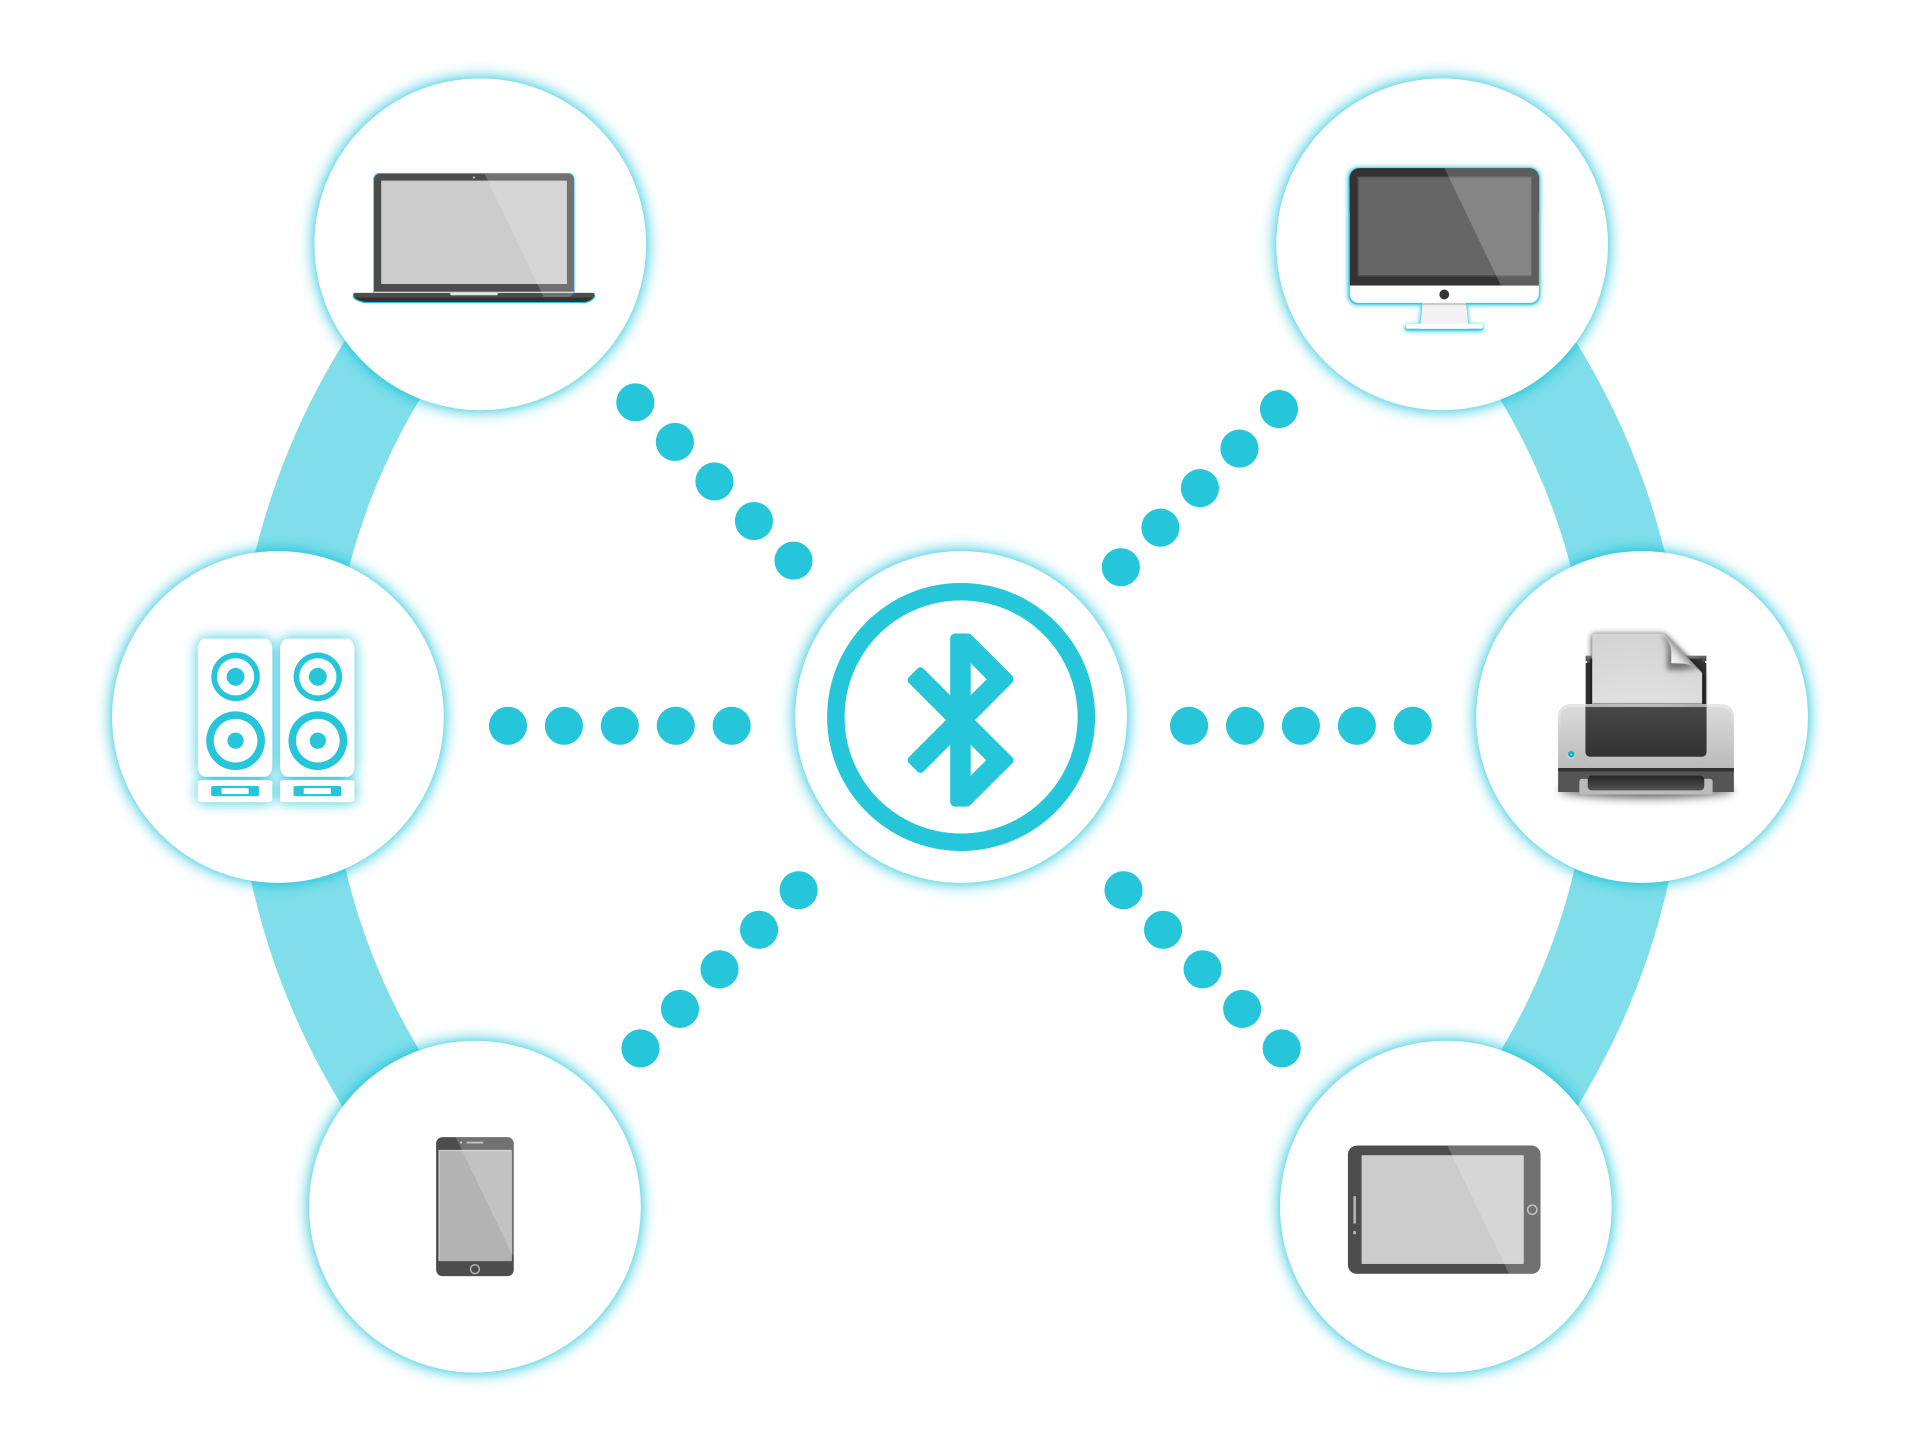
\includegraphics[width=0.7\textwidth]{img/bluetooth-ecosystem}
%    \newline Fonte: Repositório de imagens Pixabay %(link: 
%    %https://pixabay.com/en/bluetooth-connectivity-wireless-1690677/)
%\end{figure}

Uma das principais características da tecnologia \textit{wireless} é o curto alcance de 
transmissão variando de centímetros até alguns metros \cite{huang2007bluetooth}. 

A tecnologia vem sendo usada ao longo dos últimos anos em diversas aplicações como transferência de 
arquivos entre dispositivos, transmissão de áudio entre smartphones e fones sem fio, dispositivos 
capazes de determinar contexto, como os beacons, entre outros.

% Topologias
No IEEE 802.15.1 há suporte para criação de redes \textit{ad-hoc}, aos quais, é desnecessário uma 
infraestrutura de rede para conexão dos dispositivos. A partir disso é possível criar redes 
chamadas \textit{picorredes}, nas quais os dispositivos são organizados em até oito associados, 
sendo um deles um mestre, ao qual coordena as operações, e os demais escravos 
\cite{bluetoothSIG2017}.

% Características
A tecnologia Bluetooth opera na faixa ISM de 2.4 GHz de uso livre em modo TDM com 
um delta de $625\mu$s, proporcionando uma taxa de transmissão máxima em torno de 2 Mb/s, podendo 
variar de acordo com o dispositivo e a categoria de tecnologia de Bluetooth utilizada. 
\cite{bluetoothSIG2017}.

% Forma de conexão.

\subsubsection{Categorias}

Segundo \cite{sig2017}, o Bluetooth pode ser categorizado em:

\subsubsubsection{BR/EDR}
%2.0 a 2.1

% REVER
Esta é a subdivisão mais popularizada do Bluetooth presente nas versões $2.0$ e $2.1$ do Bluetooth, 
onde as principais características são alta velocidade de transmissão alta em relação à outra 
categoria, baixo alcance e necessidade de conexão através de pareamento, onde os dispositivos 
confirmam a conexão. A partir disso, há um transmissão contínua de dados. 
Uma desvantagem é o consumo de energia considerável para o funcionamento do Bluetooth, já que há 
uma conexão contínua e uma taxa de transmissão que mantêm o dispositivo ativo por um longo 
período ininterrupto.
% taxa de dados
A taxa de transmissão gira em torno de 2Mb/s.
 
\subsubsubsection{BLE (Smart)}
% 4.0, 4.1, 4.2

% O que é
O \textit{Bluetooth Low Energy} (BLE) é a mais recente categoria do Bluetooth incorporada 
na versão 4.0, em 2011, além de ser a menos comum \cite{linklabs2015}.
% Foco
BLE está centrado no baixo consumo de energia para permitir que certos 
dispositivos não precisem recarregar ou trocar suas fontes de carga, muitas vezes uma bateria, por 
longos períodos, que podem chegar a anos. 
% Pareamento
Para uma conexão para transmissão de dados, ao contrário do BR/EPR, não é necessário um pareamento 
para realizá-la, além disso esta tem curta duração, na ordem de milissegundos.
%Taxa e alcance
Ademais, a taxa de dados é baixa e o alcance alto. A baixa taxa de dados decorre do modo de 
funcionamento dos dispositivos BLE, aos quais, enviam dados em rajadas, ou seja, de tempos em 
tempos dados são transmitidos em forma de \textit{broadcast} e os dispositivos que estiverem 
conectados receberão esses dados. Nos intervalos de tempo em que o dispositivo não transmite, ele 
``dorme'', isto é, entra em modo de consumo mínimo a fim de poupar energia.

%Aplicação
A aplicação prática dessas características está na IoT através de \textit{beacons} e  
\textit{wearables}, aos quais incorporam o BLE. Os beacons foram introduzidos pela \textit{Apple} 
em conjunto com o iOS 7, com o nome de \textit{iBeacon}, que permitia aos aplicativos 
possuíssem senso de localização \cite{apple2014}. 
Com esses dispositivos é possível 
aprimorar a experiência do usuário em estabelecimentos como museus, supermercados, shoppings, 
estádios, através da identificação de contexto, na qual, a partir da 
detecção de um beacon e da aproximação ou afastamento deste, uma aplicação móvel em um smartphone 
de um usuário pode exibir conteúdos, indicar promoções entre outros relacionados aquele dispositivo 
BLE.

%\begin{figure}[H]
%	\centering
%	\caption[ABC]{{\noindent Alguns exemplares de beacons}}
%	\label{fig:beacons}
%	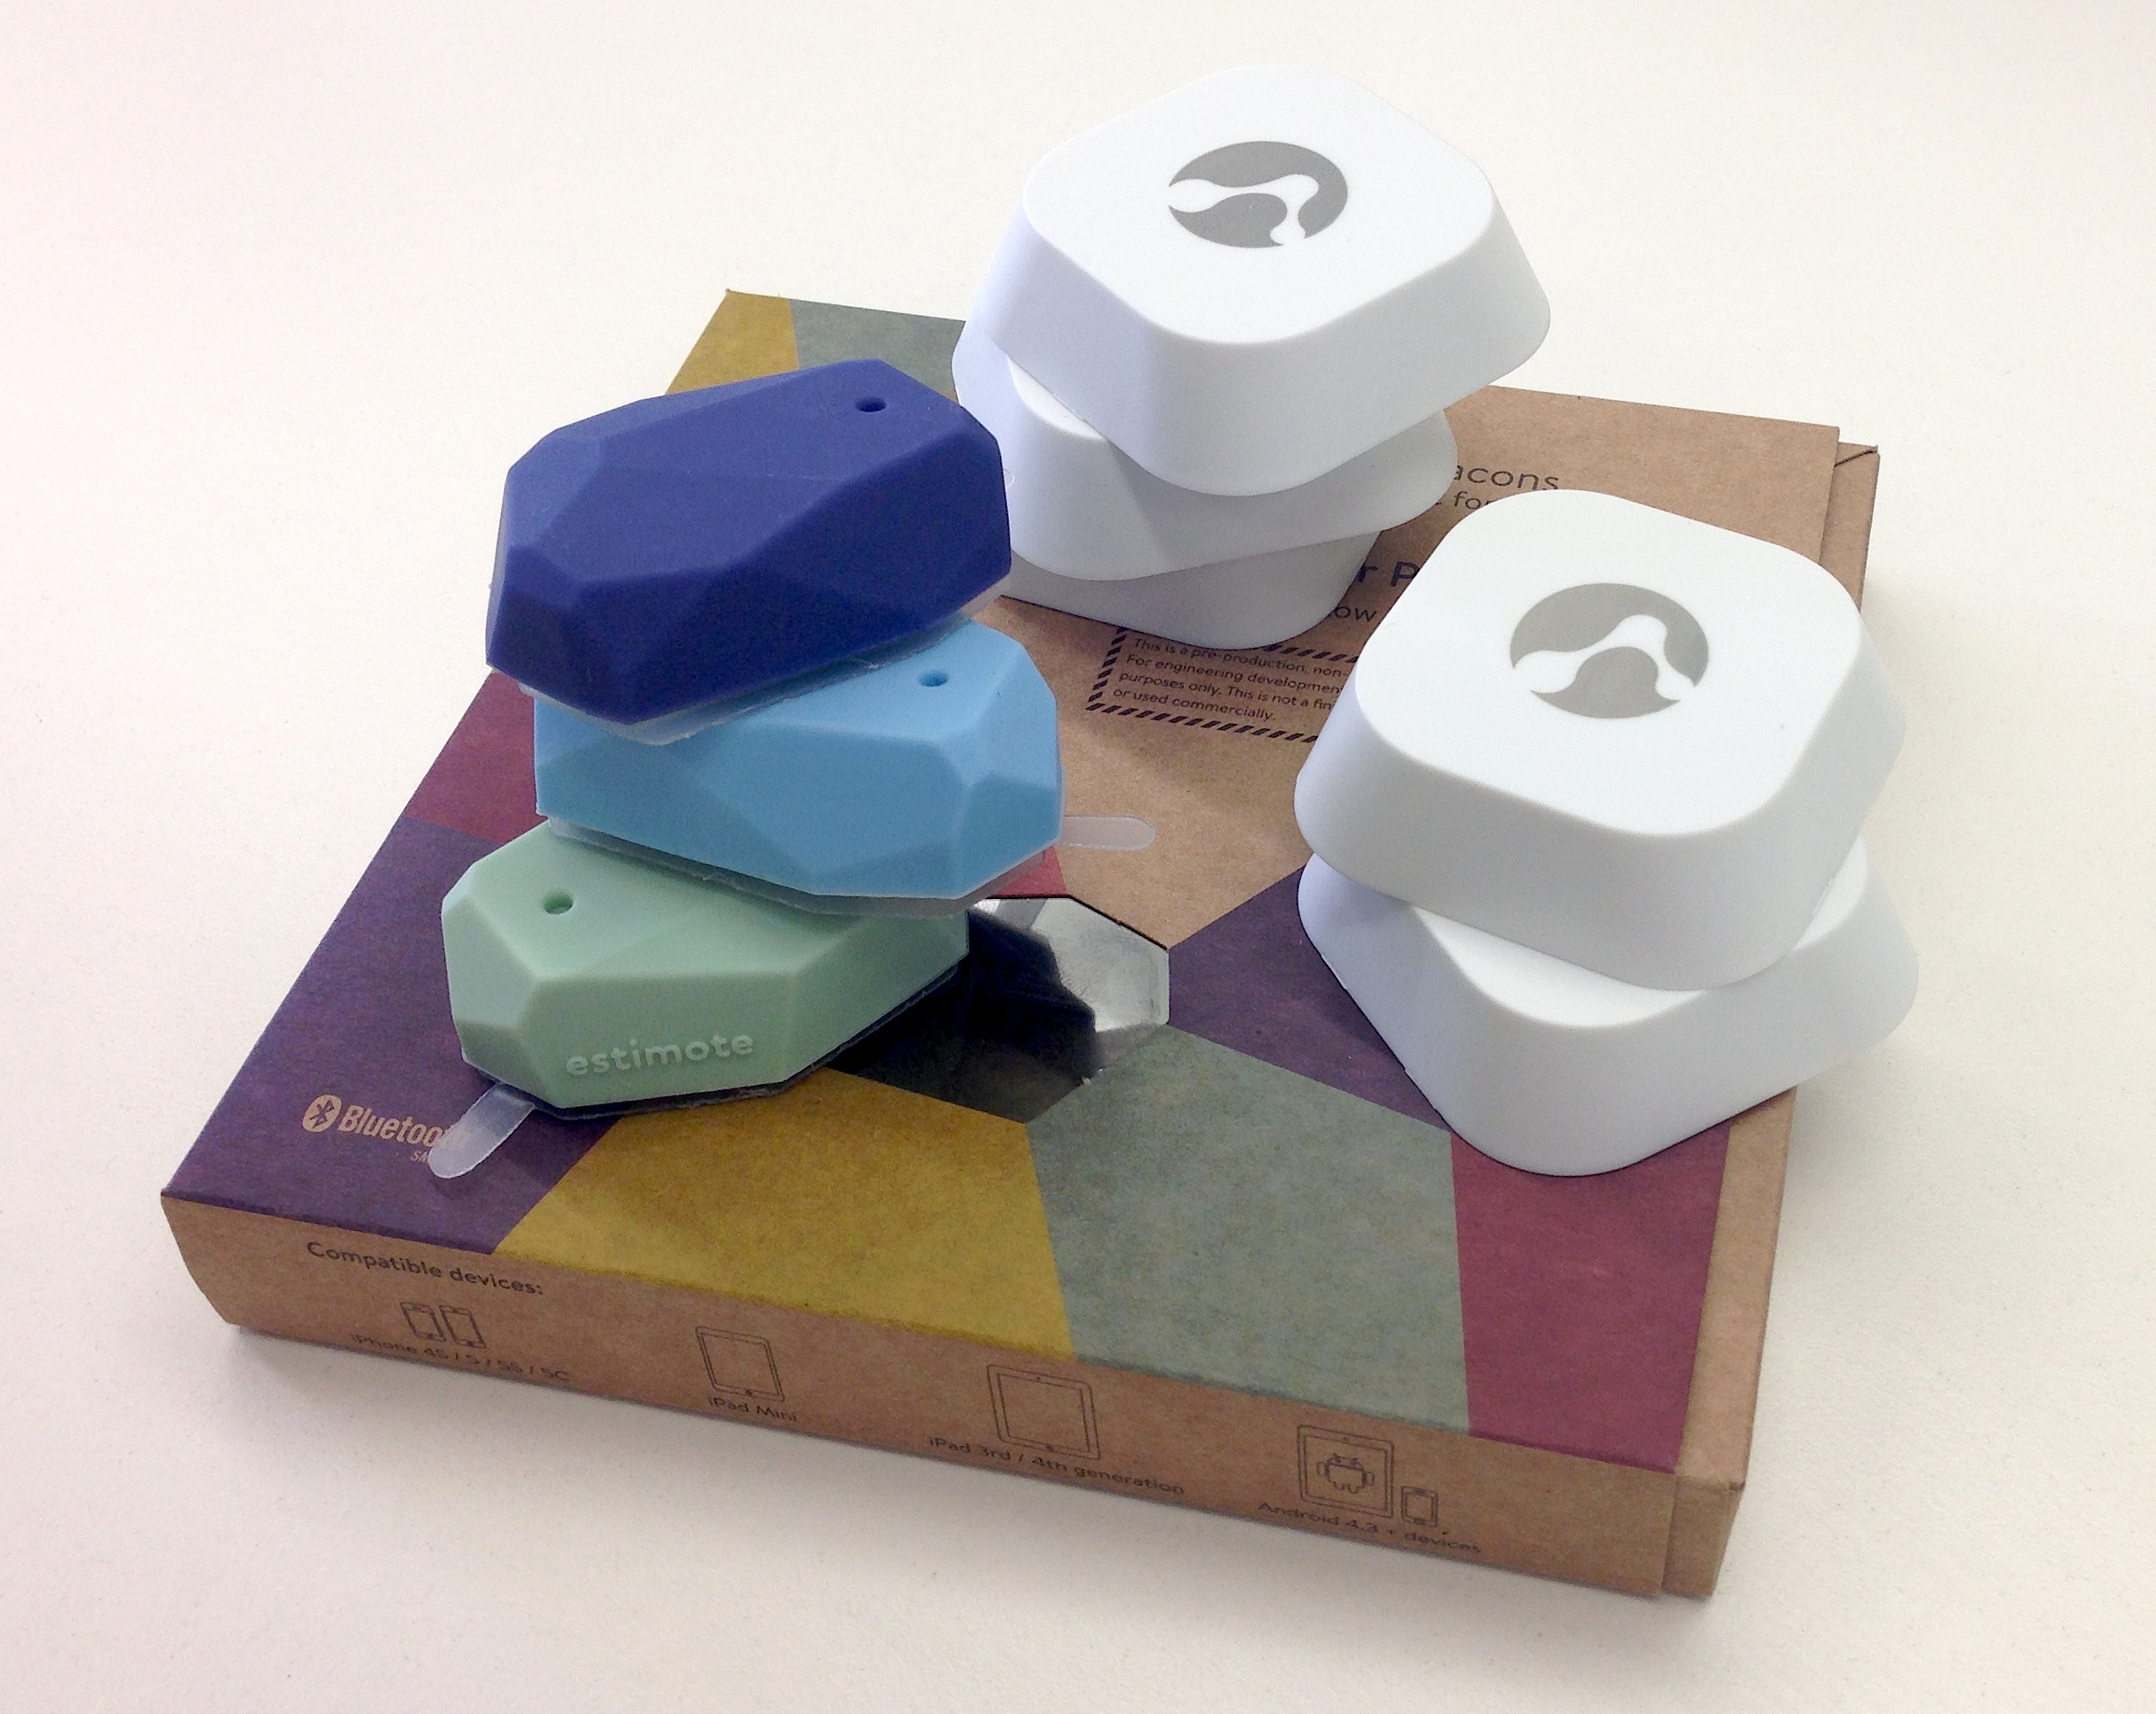
\includegraphics[width=0.5\textwidth]{img/beacons.jpg}
%	\newline Fonte: Shine Solutions %(link: 
%%https://shinesolutions.com/2014/02/17/the-beacon-experiments-low-energy-bluetooth-devices-in-action/
%\end{figure}

\subsubsubsection{Dual-mode}
%
Esta categoria se refere a dispositivos, como \textit{smartphones} que precisam 
se conectar tanto com dispositivos BR/EDR, como fones de ouvido, e BLE, como 
\textit{beacons} \cite{sig2017}.

\subsubsection{Bluetooth 5.0}

A versão 5.0 do Bluetooth foi lançada em dezembro de 2016 (adopted-specfi) e trás consigo 
aprimoramentos em desempenho e segurança, garantindo duas vezes mais velocidade, quatro vezes mais 
alcance, oito vezes mais taxa de dados e, por fim, maior coexistência \cite{bluetoothsig2016}. 

Com a nova versão, veio a flexibilidade para construção de soluções baseadas em necessidade. 
Parâmetros como alcance, velocidade e segurança podem ser regulados para diversos objetivos a 
depender das aplicações \cite{bluetoothsig2016}.

Algumas atualizações contribuem para a redução de interferência com outras tecnologias sem fio, 
dessa forma, proporciona melhor coexistência entre dispositivos Bluetooth e de outras tecnologias, 
dentro do cenário emergente da IoT \cite{bluetoothsig2016}.






% ==================================================================================================
\subsection{RFID}

O RFID (Indentificação por Rádio Frequência) é uma tecnologia de identificação automática, entre 
diversas outras como código de barras, cartão inteligente e procedimentos biométricos, no entanto 
se distingue pelo modo de funcionamento, ou seja, por ondas 
eletromagnéticas. 
% INFLUÊNCIA EXTERNAS NO FUNCIONAMENTOS
Por outro lado, o RFID se destaca em relação às outras tecnologias em relação às 
influências externas no seu funcionamento, como sujeira, posição de leitura. Desse modo, não é 
necessário nem limpar ou reposicionar o dispositivo RFID para efetuar a leitura. (rfidhandbook)

% LEITOR E TRANSPONDER
No RFID, os dados são transmitidos através de ondas de rádio entre dois dispositivos: 
\textit{transponder} ou \textit{tag} e \textit{leitor}. O transponder é localizado no objeto 
identificado, um 
produto, equipamento etc., e nele são mantidos os dados de identificação. Já o leitor é responsável 
pela leitura e escrita dos dados presentes no transponder.

% FUNCIONAMENTO
Para a transmissão dos dados entre os dois dispositivos o leitor emite ondas de rádio na tag. Ao 
receber o estímulo, a tag responde com os dados contidos nela. Além disso, existem tags que 
utilizam a energia do campo eletromagnético gerado pelo leitor para seu funcionamento, sendos estas 
chamadas de \textit{passivas}. Existem, também, aquelas que possuem uma fonte própria de energia e 
por isso são denominadas \textit{ativas}.

Um exemplo de tag ativa é mostrada na Figura \ref{fig:active-rfid}.

%\begin{figure}[H]
%	\centering
%	\caption[ABC]{{\noindent Exemplo tag RFID ativa}}
%	\label{fig:active-rfid}
%	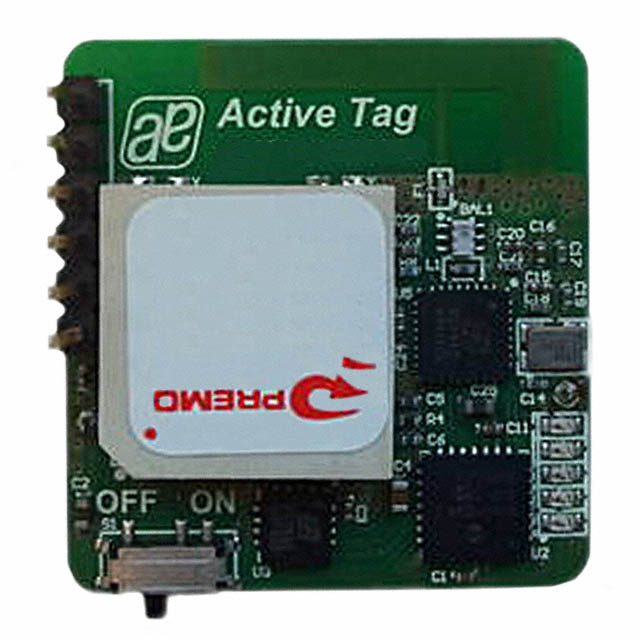
\includegraphics[width=0.3\textwidth]{img/active-tag.jpg}
%	\newline Fonte: Vnsky %(link: 
%	%http://www.vnsky.com/parts/2673180/ACTIVE-TAG-REFERENCE-DESIGN-KIT.html
%\end{figure}

Uma tag passiva é mostrada na Figura \ref{fig:passive-rfid}.

%\begin{figure}[H]
%	\centering
%	\caption[ABC]{{\noindent Exemplo tag RFID passiva}}
%	\label{fig:passive-rfid}
%	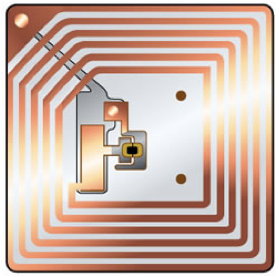
\includegraphics[width=0.3\textwidth]{img/passive.png}
%	\newline Fonte: Eletrosome %(link: 
%	%https://electrosome.com/rfid-radio-frequency-identification/
%\end{figure}

% TIPOS (alimentação)

% ATIVO
% PASSIVO

% FREQ. DE OPERAÇÃO
Uma das características mais importante dos dispositivos RFID é a frequência de operação já que ela 
influi no distância máxima de operação. Tal fator é determinado pelo leitor. 

Os dispositivos são classificados, de acordo com a frequência de operação, em três grupos:

\begin{itemize} \parskip -4pt
	\item \textbf{LF (Baixa Frequência):} Entre 30kHz à 300kHz
	\item \textbf{HF (Alta Frequência):} Entre 3MHz à 30MHz
	\item \textbf{UHF (Ultra Alta Frequência)}: Entre 300MHz a 3GHz.
\end{itemize}

É possível distinguir pelo alcance:

\begin{itemize} \parskip -4pt
	\item \textbf{\textit{Long-range} ou longo alcance:} maior que um metro.
	\item \textbf{\textit{Remote-coupling} ou ligação remota:} até um metro
	\item \textbf{\textit{Close-coupling} ou ligação próxima:} até um centímetro.
\end{itemize}

Geralmente, a frequência de operação é diretamente proporcional ao alcance. Por exemplo, 
dispositivos de longo alcance operam na faixa UHF. 






% ==================================================================================================
\subsection{NFC}
% O_QUE É
O NFC é um sistema de comunicação sem fio derivado do RFID. Ele permite transações simples e 
seguras entre dois dispositivos a partir da curta distância de operação, em torno de 
4cm, e do funcionamento baseado em aproximação dos objetos em questão \cite{nfcforumabout2017}. 
Assim, é 
possível realizar leituras de tags e obter conteúdos de acordo com a aplicação, transferir dados 
entre smartphones entre outras funcionalidades.

% COMPATIBILIDADE
Outra vantagem do NFC é a compatibilidade com a infraestrutura de cartões sem contato 
existentes permitindo usar um único dispositivo em tecnologias diferentes. Desse modo, é possível 
interagir com tags RFID, por exemplo.


% FUNCIONAMENTO
Como o RFID, o NFC funciona através de ondas eletromagnéticas com uma taxa de transmissão máxima de 
424kbps \cite{nfcforumabout2017}. Além disso, pode operar em dois modos de comunicação 
\cite{brianjepsondoncolemantomigoe2014}: ativo e passivo. Assim como no RFID, é possível que os 
dispositivos NFC que contenham 
os dados usema energia do leitor para transmitir seus dados, no modo passivo ou usem uma fonte 
própria para tal procedimento, no modo ativo.


% MODOS DE OPERAÇÃO
Outra característica importante no NFC são os modos de operação. De acordo com (NFC-forum) existem 
três modos de operação:

\begin{itemize} \parskip -4pt
	\item \textit{Leitor/Escritor de tag}: Tem por objetivo ligar o mundo físico ao digital através 
	de aplicações que leem e/ou escrevem em tags para obter dados e, assim, fornecer conteúdo ao 
	usuário relacionado à tag lida. Um exemplo é um smartphone ao ler uma tag NFC de um cartaz na 
	rua.
	\item \textit{Peer to Peer}: Visa conectar dispositivos por aproximação física e permite troca 
	de arquivos. Um exemplo é o Android Beam que permite troca de arquivos entre smartphones com o 
	sistema operacional da Google.
	\item \textit{Emulação de cartão}: Conecta o dispositivo do usuário em uma infraestrutura 
	possibilitando a simulação de um cartão, além da realização de transações financeiras e 
	identificação no sistema de transporte a partir da aproximação do dispositivo a um leitor 
	específico.
\end{itemize}

% CATEGORIAS
Há quatros tipos de tags definidas \cite{nfcforumtypespec2017}, sendo que todos operam no modo 
Leitor/Escritor descrito anteriorente : 

\begin{itemize} \parskip -4pt
	\item \textbf{Tipo 1}: 96 bytes de memória disponível e expansível para 2kiB. Usuário pode 
	configurá-la para somente leitura.
	\item \textbf{Tipo 2}: 48 bytes de memória disponível e expansível para 2kiB. Usuário pode 
	configurá-la para somente leitura.
	\item \textbf{Tipo 3}: Baseado no padrão industrial japonês e conhecido como FeliCa. Pode ser 
	configuradas para leitura/escrita ou somente leitura na fabricação. A memória disponível varia, 
	mas com um limite teórico de 1MiB por serviço.
	\item \textbf{Tipo 4}: A memória disponível varia estando acima de 35 kiB por serviço. É 
	possível ser configurada para leitura/escrita ou somente leitura.
\end{itemize}

O NFC possui um padrão com o qual dispositivos devem estar formatados, o NDEF (\textit{NFC Data 
Exchange Format}) um formato comum de comunicação \cite{brianjepsondoncolemantomigoe2014}. Desse 
modo, os dados 
armazenados em tags devem estar gravados nesse formato. A partir do NDEF é possível 
armazenar e trocar documentos binários como MIME, que incluem imagens, arquivos PDF entre outros, 
URL, texto simples entre outros.







% ==================================================================================================
\subsection{Zigbee}


\section{Aplicações}

Pouco tempo após à primeira referência a IoT, em 2000, uma empresa de grande porte, a LG, lançou 
um produto baseado na ideia de IoT: uma geladeira capaz de verificar se os produtos contidos nela 
foram reabastecidos \cite{survey-suresh}.



% TODO: PRESENTE
Atualmente, a IoT evoluiu e já está presente em diversos setores como 

% Smart home
% Smart grid
% Indústrias
% Transportes


% TODO: FUTURO


%%%%%%%%%%%%%%%%%%%%%%%%%%%%%%%%%%%%%%%%%%%%%%%%%%%%%%%%%%%%%%%%%
% ---
% Finaliza a parte no bookmark do PDF, para que se inicie o bookmark na raiz
% ---
\bookmarksetup{startatroot}% 
% ---

% ---
% Conclusão
% ---
\section*{Considerações finais}
\addcontentsline{toc}{section}{Considerações finais}





% ]  				% FIM DE ARTIGO EM DUAS COLUNAS
% ---

% ----------------------------------------------------------
% Referências bibliográficas
% ----------------------------------------------------------
\bibliography{ref}


\end{document}
